% ===== Shared manuscript body (identical content for IEEE and Springer versions) =====
\begin{abstract}
Accurate ab initio gene prediction is the first step of genome annotation, yet widely used self-training gene finders such as Prodigal and its Python port Pyrodigal are tuned for bacterial chromosomes and can degrade on short, AT-rich or organellar genomes. We (i) benchmark Pyrodigal in its single-genome (self-trained) and metagenomic modes against RefSeq annotation on three real, fully annotated genomes (the 154~kb \textit{Arabidopsis thaliana} chloroplast, the \textit{Yersinia pestis} plasmid pPCP1 and phage phiX174), and (ii) propose \emph{CodonRescore}, a lightweight, annotation-free post-processor that re-scores every gene call with a 3-periodic order-2 Markov codon model trained on the genome's own long ORFs, with a decision threshold obtained from a cross-fitted comparison of seed ORFs against shadow-frame ORFs. On the chloroplast genome, self-trained Pyrodigal calls 43 false genes (precision 0.574, F1 0.678); CodonRescore prunes 38 calls (35 of them false) and raises precision to 0.778 and F1 to 0.789 at a cost of 2 true genes. Applied to Pyrodigal's metagenomic mode, which is already strong (F1 0.841), CodonRescore does not help (F1 0.816; bootstrap intervals overlap). A 2.46~Mb \textit{Corynebacterium diphtheriae} genome shows the method scales and behaves consistently (45 pruned, 69 rescued calls, all short). We discuss the limits of this small benchmark and outline extensions using protein language models.
\end{abstract}

\begin{keywords}
Gene prediction; ORF; codon usage; Markov model; Pyrodigal; chloroplast genome; genome annotation; computational biology
\end{keywords}

\section{Introduction}
Gene prediction converts a raw genome sequence into a catalogue of protein-coding genes and underlies comparative genomics, pathway reconstruction and the interpretation of variants. Prokaryotic and organellar genomes are gene dense, so the task is conceptually simple---find long open reading frames (ORFs) with coding statistics---but remains error prone for short genes, atypical (horizontally transferred or AT-rich) genes, overlapping genes and translation-initiation-site selection. Annotation pipelines such as Bakta~\cite{schwengers2021} still delegate coding-sequence (CDS) discovery to Prodigal~\cite{hyatt2010}, here accessed through its maintained Python port Pyrodigal~\cite{larralde2022}, so errors of this first stage propagate to every downstream annotation.

Recent work has pushed accuracy in two directions: broad benchmarks showing that no single tool is best across organisms~\cite{dimonaco2022}, and machine-learning models that classify ORFs, from the universal protein model of Balrog~\cite{sommer2021} to protein-language-model classifiers for short genes~\cite{tu2023}. These models require large training corpora and, often, GPUs. For a student- or laboratory-scale workflow, a cheap check that can be bolted onto any gene caller and trained only on the genome at hand is attractive.

This paper contributes (1) a transparent benchmark of Pyrodigal's two operating modes against real RefSeq annotation on small genomes where self-training is difficult; (2) \emph{CodonRescore}, an annotation-free codon-model rescoring procedure with an unsupervised threshold; and (3) a critical analysis, including a negative result, of when rescoring helps.

\section{Literature Review / Related Work}
We reviewed seven recent papers (2021--2024) together with three foundational or context references. Table~\ref{tab:lit} summarises the approaches, data and limitations that motivate this study.

\begin{table}[t]
\caption{Summary of reviewed literature (recent works, 2021--2024).}\label{tab:lit}
\centering\footnotesize
\resizebox{\linewidth}{!}{%
\begin{tabular}{p{0.9cm}p{0.5cm}p{3.6cm}p{3.4cm}p{3.6cm}}
\toprule
Ref. & Year & Approach & Data / scope & Limitation relevant here \\
\midrule
\cite{larralde2022} & 2022 & Cython port of Prodigal (dynamic programming over ORFs, self-trained GC-frame and start-site models; metagenomic mode with pre-trained models) & Bacterial/archaeal genomes, metagenomes & Needs sufficient sequence (here $\geq$20~kb) to self-train; no organelle-specific model \\
\cite{sommer2021} & 2021 & Balrog: temporal convolutional network scoring ORFs as protein-like, trained once on many genomes & Diverse bacterial genomes & Heavy pre-training; fewer calls than Prodigal at similar sensitivity; not organelle-focused \\
\cite{dimonaco2022} & 2022 & Benchmark of several prokaryotic gene finders against reference annotation & Many genomes across taxa & Performance is organism dependent; short and atypical genes are missed or over-called \\
\cite{schwengers2021} & 2021 & Bakta: annotation pipeline; CDS from Prodigal plus alignment-free sequence identification & Bacterial genomes & Inherits upstream CDS errors \\
\cite{tu2023} & 2023 & ProtiGeno: ESM-1b protein-language-model embeddings classify short ORFs & 4,288 genomes; short genes ($<180$~nt) & Higher recall at lower precision; needs large pre-trained model \\
\cite{gabriel2024} & 2024 & BRAKER3: evidence integration (RNA-seq, proteins) with GeneMark-ETP, AUGUSTUS and TSEBRA selection & Eukaryotic genomes & Needs external evidence; eukaryote focus (relevant as an ensembling principle) \\
\cite{zhou2024} & 2024 & DNABERT-2: multi-species DNA foundation model with byte-pair tokenisation and a benchmark & Multi-species genomes; classification tasks & General-purpose; not evaluated for gene-boundary calling \\
\bottomrule
\end{tabular}}
\end{table}

\textbf{Existing approaches.} Classical gene finders combine a coding-statistics model (a periodic Markov chain or hexamer statistics) with start-site models and dynamic programming; Prodigal~\cite{hyatt2010} trains these unsupervised on the input genome, whereas its metagenomic mode uses precomputed models selected per sequence~\cite{larralde2022}. Learning-based approaches replace hand-crafted statistics by neural classifiers of translated ORFs~\cite{sommer2021,tu2023}. Evidence-driven eukaryotic pipelines illustrate the value of reconciling several predictors~\cite{gabriel2024}, and pretrained DNA language models~\cite{zhou2024} suggest future feature extractors. \textbf{Datasets} in these works are large public genome collections (RefSeq/GenBank); we use real RefSeq records but at much smaller scale. \textbf{Chloroplast genomes} are prokaryote-like, compact and annotated by dedicated tools~\cite{tillich2017}; the \textit{A.~thaliana} plastid genome was sequenced in full in 1999~\cite{sato1999}.

\section{Research Gap}
From the reviewed works we identify three gaps. (G1) Benchmarks and models concentrate on bacterial chromosomes or large collections; the behaviour of Prodigal-style self-training on small AT-rich organellar genomes is not examined in the works we reviewed. (G2) Deep-learning ORF classifiers need large pre-training and compute, and there is little work on cheap, genome-specific post-hoc rescoring that can be combined with any caller. (G3) Published comparisons seldom separate \emph{which} errors (short ORFs, shadow frames, RNA genes) dominate false positives, so it is unclear where a rescoring step should intervene.

\section{Problem Statement}
Given a complete, unannotated DNA sequence $S$ of a prokaryotic or organellar genome and the output $G_0$ of an ab initio gene caller, produce a refined gene set $G$ that increases precision without a loss of sensitivity, using only $S$ itself (no annotation, no external training data), and quantify when this succeeds on real annotated genomes.

\section{Objectives}
\begin{enumerate}
\item To benchmark Pyrodigal (single and metagenomic modes) and a long-ORF baseline against RefSeq annotation on real small genomes.
\item To design CodonRescore, a self-trained codon-model rescoring method with an unsupervised, cross-fitted decision threshold.
\item To analyse sensitivity to the threshold and pruning length, error anatomy by gene length and by overlap with RNA genes, and statistical uncertainty.
\item To test scalability and consistency on a 2.46~Mb genome and to document limitations honestly.
\end{enumerate}

\section{Proposed Methodology}
\textbf{Overview.} CodonRescore has three stages (Fig.~\ref{fig:arch}): (1) enumerate candidate ORFs and select \emph{seed} ORFs, (2) train a periodic coding model and derive a threshold $\tau$ without annotation, (3) re-score the caller's genes: \emph{prune} short low-scoring calls and \emph{rescue} high-scoring uncalled ORFs. Evaluation uses GenBank annotation \emph{only} for scoring, never for training or tuning: $\tau$, the pruning length (300~nt), the rescue length (120~nt) and all seed parameters were fixed before the benchmark was run. Sensitivity to these settings is reported post hoc and not used to choose them.

\textbf{Evaluation protocol.} A prediction is a true positive (TP) if its strand and stop-codon coordinate match a single-exon, non-pseudo CDS (``stop match'', the customary gene-finder criterion since start sites are ambiguous); \emph{exact recall} additionally requires the start to match. Annotated multi-exon CDSs, pseudogenes and CDSs spanning the sequence origin cannot be represented by a linear ORF caller; predictions overlapping them by $\geq$50\% of their length are counted as ``neutral'' and excluded from precision. Precision $=\mathrm{TP}/(\mathrm{TP}+\mathrm{FP})$, recall $=$ matched truth genes / truth genes, F1 is their harmonic mean. 95\% confidence intervals use a bootstrap (2,000 replicates; truth genes resampled for recall, predictions for precision).

\begin{figure*}[t]
\centering
\resizebox{0.98\linewidth}{!}{%
\begin{tikzpicture}[every node/.style={font=\footnotesize},
 box/.style={draw, rounded corners=2pt, align=center, minimum height=9mm, minimum width=24mm, fill=blue!6},
 hl/.style={draw, rounded corners=2pt, align=center, minimum height=9mm, minimum width=24mm, fill=orange!18},
 ar/.style={-{Stealth[length=2mm]}, thick}]
\node[box] (seq) at (0,0) {Genome\\sequence $S$};
\node[box] (orf) at (3.8,0) {Enumerate ORFs\\both strands\\($\geq$90~nt)};
\node[hl] (seed) at (7.6,0) {Seed ORFs\\($\geq$450~nt,\\low overlap)};
\node[hl] (model) at (11.4,0) {Periodic order-2\\Markov coding\\model vs.\ background};
\node[box] (caller) at (3.8,-2.3) {Gene caller\\(Pyrodigal single/meta)\\calls $G_0$};
\node[hl] (rs) at (7.6,-2.3) {Re-score calls:\\prune short $S<\tau$,\\rescue ORFs $S\geq\tau$};
\node[hl] (tau) at (11.4,-2.3) {Threshold $\tau$ (2-fold\\Youden: seeds vs.\\shadow ORFs)};
\node[box] (out) at (7.6,-4.5) {Refined gene set $G$};
\draw[ar] (seq)--(orf); \draw[ar] (orf)--(seed); \draw[ar] (seed)--(model);
\draw[ar] (model)--(tau); \draw[ar] (tau)--(rs); \draw[ar] (caller)--(rs);
\draw[ar] (rs)--(out); \draw[ar] (seq.south) |- (caller.west);
\end{tikzpicture}}
\caption{CodonRescore architecture. Orange blocks are the proposed components; the caller is any ab initio method. No annotation is used at any stage.}\label{fig:arch}
\end{figure*}

\section{Dataset / Database Description}
All sequences are real, publicly archived NCBI records distributed with open-source software test suites (Biopython 1.85 and Pyrodigal 3.7.1) and were used unmodified (Table~\ref{tab:data}). The truth sets are the RefSeq CDS annotations of three records. The 2.46~Mb \textit{C.\ diphtheriae} chromosome has no annotation in our files and is used only to examine scalability and agreement between methods, not accuracy.

\begin{table}[t]
\caption{Datasets. $^\dagger$Neutral = parts of multi-exon CDSs, pseudogenes and genes spanning the origin (three phiX174 genes); excluded from precision.}\label{tab:data}
\centering\footnotesize
\resizebox{\linewidth}{!}{\begin{tabular}{llrrcl}
\toprule
Accession & Organism / record & Length (bp) & GC (\%) & CDS: all / eval. / neutral$^\dagger$ & Role \\
\midrule
NC\_000932.1 & \textit{A. thaliana} chloroplast & 154,478 & 36.3 & 85 / 70 / 34 & Truth + training \\
NC\_005816.1 & \textit{Y. pestis} plasmid pPCP1 & 9,609 & 45.3 & 10 / 10 / 0 & Truth \\
NC\_001422.1 & Coliphage phiX174 & 5,386 & 44.8 & 11 / 8 / 6 & Truth \\
NZ\_LN831026.1 & \textit{C. diphtheriae} NCTC11397 & 2,463,666 & 53.5 & not used & Agreement only \\
\bottomrule
\end{tabular}
}
\end{table}

The chloroplast record has 85 annotated CDSs, of which 70 are single-exon and usable as truth; 15 are spliced and treated as neutral (34 exon parts). The record also contains 37 tRNA and 7 rRNA genes, which matter for the false-positive analysis. The pPCP1 and phiX174 genomes are very small and therefore also test the failure mode of self-training with too few seeds.

\section{System / Methodology Architecture}
The implementation is a pure-Python/NumPy module (\texttt{codonrescore.py}) plus an evaluation harness; the only external gene caller is Pyrodigal~3.7.1. Fig.~\ref{fig:arch} shows the data flow. Every stage is deterministic given the sequence; the bootstrap uses a fixed random seed (2026).

\section{Algorithms / Computational Methods}
\textbf{ORF enumeration.} For each strand and frame, consecutive stop codons (TAA, TAG, TGA; translation table~11) delimit stretches; the most upstream ATG/GTG/TTG in a stretch defines the longest ORF for that stop. ORFs with length $\geq 90$~nt are candidates.

\textbf{Coding score.} Let $o=x_1\ldots x_n$ be an ORF in the coding direction. A coding model $P_c(x_i\mid x_{i-2}x_{i-1},\,i \bmod 3)$ and a homogeneous background model $P_b(x_i\mid x_{i-2}x_{i-1})$ (both order-2 with Laplace smoothing, $\alpha=1$) give the per-codon log-likelihood ratio
\begin{equation}
S(o)=\frac{3}{n}\sum_{i=3}^{n}\Big[\log P_c(x_i\mid x_{i-2}x_{i-1},\,i\bmod 3)-\log P_b(x_i\mid x_{i-2}x_{i-1})\Big].
\end{equation}
$P_b$ is estimated from both strands of the whole genome (a neutral reference), $P_c$ from the seed ORFs.

\begin{algorithm}[t]
\caption{CodonRescore training (annotation-free)}\label{alg:train}
\begin{algorithmic}[1]
\Require genome $S$
\State $\mathcal{O}\gets$ ORFs$(S,\ \ge 90)$
\State $\mathcal{S}\gets$ greedy longest-first ORFs $\ge 450$~nt overlapping accepted seeds by $\le 30\%$ (relax to 360, then 300~nt if $<10$ seeds; fail if still $<10$)
\State split $\mathcal{S}$ into folds $A,B$ (alternating)
\For{$k\in\{A,B\}$}
  \State fit $P_c$ on the other fold, $P_b$ on $S$ and $\overline{S}$
  \State score held-out seeds (positives) and shadow ORFs (negatives: ORFs overlapping a held-out seed by $\ge 50\%$ of their length in another frame)
\EndFor
\State $\tau\gets\arg\max_t\ [\,\mathrm{TPR}(t)+\mathrm{TNR}(t)-1\,]$ (Youden)
\State refit $P_c$ on all seeds \Return $(P_c,P_b,\tau)$
\end{algorithmic}
\end{algorithm}

\begin{algorithm}[t]
\caption{CodonRescore re-scoring of a gene set $G_0$}\label{alg:rescore}
\begin{algorithmic}[1]
\State \textbf{prune:} remove $g\in G_0$ if $S(g)<\tau$ \textbf{and} $|g|<300$~nt
\State \textbf{rescue:} for ORFs $c$ with $|c|\ge120$ and $S(c)\ge\tau$, in decreasing total score, add $c$ unless it overlaps a kept gene by $>60$~nt (same strand) or by $>60\%$ of the shorter gene (opposite strand)
\State \Return kept $\cup$ rescued
\end{algorithmic}
\end{algorithm}

Two further variants are reported: \emph{CodonLLR-only} (all ORFs with $S\ge\tau$ after greedy conflict resolution by total score) and a \emph{LongORF$\ge$300} baseline. \emph{CodonRescore(single)} and \emph{(meta)} apply Algorithm~\ref{alg:rescore} to Pyrodigal single-mode and metagenomic-mode output, respectively.

\section{Experimental Setup}
Software: Python~3.13, NumPy, Biopython~1.88 (parsing), Pyrodigal~3.7.1 (default parameters; single mode trained on the same sequence it annotates; metagenomic mode with its built-in models), Matplotlib. Pyrodigal single mode requires $\geq$20~kb and is therefore not run on pPCP1 and phiX174. CodonRescore failed its seed requirement on phiX174 (only 5 non-overlapping ORFs $\geq$300~nt) and is reported as not applicable there. Runtime on a single CPU core was about 37~s for the full analysis including the 2.46~Mb genome. All code and result files are provided with the submission.

\section{Results and Analysis}
\textbf{Main benchmark (chloroplast).} Table~\ref{tab:chloro} and Fig.~\ref{fig:f1} summarise the 70 evaluable genes. Pyrodigal in single mode recovers 58 of 70 genes but emits 43 false positives (precision 0.574, F1 0.678). The metagenomic mode is markedly better (precision 0.813, recall 0.871, F1 0.841). CodonRescore applied to the single-mode output removes 38 calls, of which only 3 were true genes, and rescues 9 ORFs (1 true); precision rises to 0.778 and F1 to 0.789. Applied to the metagenomic mode, it prunes 9 calls (1 true) and rescues 10 (0 true), leaving F1 at 0.816 versus 0.841.

\begin{table}[t]
\caption{Chloroplast genome (70 evaluable CDS). Neut.\ = neutral predictions excluded from precision; exact rec.\ = start and stop match.}\label{tab:chloro}
\centering\footnotesize
\resizebox{\linewidth}{!}{\begin{tabular}{lrrrrrrrl}
\toprule
Method & Pred. & TP & FP & Neut. & Prec. & Rec. & Exact rec. & F1 [95\% CI] \\
\midrule
LongORF$\geq$300 & 71 & 45 & 11 & 15 & 0.804 & 0.643 & 0.429 & 0.714 [0.63--0.79] \\
Pyrodigal-single & 122 & 58 & 43 & 21 & 0.574 & 0.829 & 0.643 & 0.678 [0.59--0.75] \\
Pyrodigal-meta & 97 & 61 & 14 & 22 & 0.813 & 0.871 & 0.743 & 0.841 [0.78--0.90] \\
CodonLLR-only & 105 & 60 & 23 & 22 & 0.723 & 0.857 & 0.614 & 0.784 [0.72--0.84] \\
CodonRescore(single) & 93 & 56 & 16 & 21 & 0.778 & 0.800 & 0.614 & 0.789 [0.72--0.85] \\
CodonRescore(meta) & 98 & 60 & 17 & 21 & 0.779 & 0.857 & 0.729 & 0.816 [0.75--0.88] \\
\bottomrule
\end{tabular}
}
\end{table}

\begin{figure}[t]
\centering
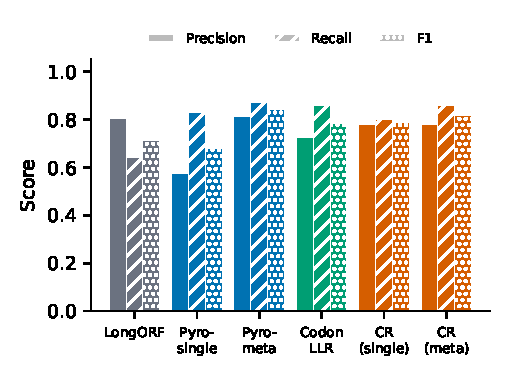
\includegraphics[width=0.95\linewidth]{../figs/fig_f1_bars.pdf}
\caption{Precision, recall and F1 on the chloroplast genome. CR = CodonRescore.}\label{fig:f1}
\end{figure}

\textbf{Statistical uncertainty.} The F1 intervals of Pyrodigal-single [0.59--0.75] and CodonRescore(single) [0.72--0.85] overlap, as do those of Pyrodigal-meta [0.78--0.90] and CodonRescore(meta) [0.75--0.88]. With 70 truth genes, the F1 gains are therefore suggestive rather than statistically established, whereas the precision change for single mode (43 $\rightarrow$ 16 false positives) is large in absolute terms.

\textbf{All genomes.} Table~\ref{tab:all} shows the small genomes. On pPCP1 (10 genes) Pyrodigal-meta is best (F1 0.947); CodonRescore(meta) reaches recall 1.0 by rescuing one true gene but adds three false calls (precision 0.769), and CodonLLR-only is poor (F1 0.692). On phiX174, Pyrodigal-meta finds 6 of 8 evaluable genes with no false positives; a 5~kb genome gives too few seeds for any self-trained codon model.

\begin{table}[t]
\caption{Precision (P), recall (R) and F1 on all truth genomes. ``--'': method not applicable (size or seed requirement).}\label{tab:all}
\centering\footnotesize
\resizebox{\linewidth}{!}{\begin{tabular}{lccccccccc}
\toprule
Method & \multicolumn{3}{c}{Chloroplast} & \multicolumn{3}{c}{pPCP1 plasmid} & \multicolumn{3}{c}{phiX174} \\
& P & R & F1 & P & R & F1 & P & R & F1 \\
\midrule
LongORF$\geq$300 & 0.804 & 0.643 & 0.714 & 0.900 & 0.900 & 0.900 & 0.500 & 0.625 & 0.556 \\
Pyrodigal-single & 0.574 & 0.829 & 0.678 & -- & -- & -- & -- & -- & -- \\
Pyrodigal-meta & 0.813 & 0.871 & 0.841 & 1.000 & 0.900 & 0.947 & 1.000 & 0.750 & 0.857 \\
CodonLLR-only & 0.723 & 0.857 & 0.784 & 0.562 & 0.900 & 0.692 & -- & -- & -- \\
CodonRescore(single) & 0.778 & 0.800 & 0.789 & -- & -- & -- & -- & -- & -- \\
CodonRescore(meta) & 0.779 & 0.857 & 0.816 & 0.769 & 1.000 & 0.870 & -- & -- & -- \\
\bottomrule
\end{tabular}
}
\end{table}

\textbf{Score separation.} The cross-fitted per-codon LLR separates held-out seed ORFs from shadow-frame ORFs well on the chloroplast genome (Youden $J=0.909$, $\tau=0.025$; 50 seeds, 470 shadow ORFs; Fig.~\ref{fig:llr}), which explains the reliable pruning of spurious calls.

\begin{figure}[t]
\centering
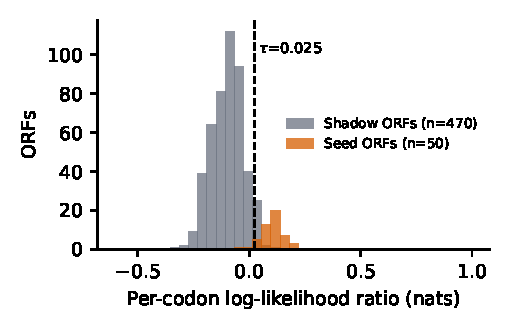
\includegraphics[width=0.95\linewidth]{../figs/fig_llr.pdf}
\caption{Cross-fitted per-codon LLR of seed ORFs versus shadow-frame ORFs, chloroplast genome. Dashed line: $\tau$.}\label{fig:llr}
\end{figure}

\textbf{Error anatomy.} Of the 43 false positives of Pyrodigal-single, 38 are shorter than 300~nt (median length 225~nt), 24 overlap an annotated tRNA or rRNA gene, and none overlaps a true protein gene in another frame. Self-training on a genome in which RNA genes and non-coding sequence make up a large fraction of the sequence thus appears to relax the coding model; this is consistent with the strong gain from a length-aware prune. Length-stratified recall (Fig.~\ref{fig:len}) shows that all methods recover all 29 genes $\geq$600~nt and at least 15 of the 16 genes of 300--599~nt; differences arise mainly in the 25 genes $<$300~nt, where recall is 14/25 (single), 16/25 (meta), 12/25 (CodonRescore, single) and 15/25 (CodonRescore, meta).

\begin{figure}[t]
\centering
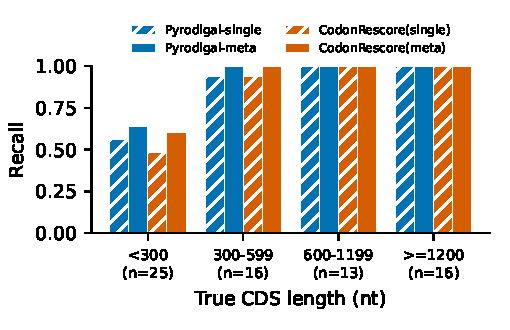
\includegraphics[width=0.95\linewidth]{../figs/fig_lenrecall.pdf}
\caption{Recall by true CDS length (chloroplast).}\label{fig:len}
\end{figure}

\textbf{Sensitivity analysis.} Fig.~\ref{fig:sens} and Table~\ref{tab:sens} show the effect of shifting the unsupervised threshold post hoc. Lowering $\tau$ by 0.1 or more is catastrophic (F1 $<$0.44) because many weakly coding ORFs are rescued; raising it trades recall for precision (F1 0.74--0.79). Pruning length matters less: with a 450-nt rule, F1 rises to 0.800 (single) and 0.825 (meta), still below unmodified Pyrodigal-meta (0.841). These values were not used to choose parameters; doing so on the same 70 genes would overfit.

\begin{figure}[t]
\centering
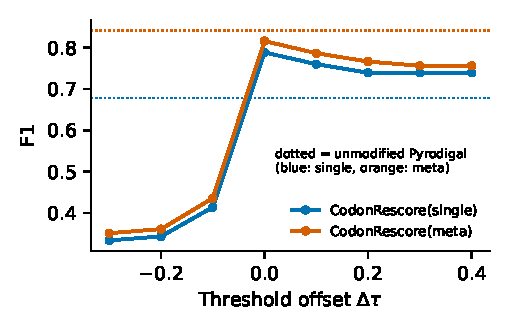
\includegraphics[width=0.95\linewidth]{../figs/fig_sens.pdf}
\caption{F1 as a function of threshold offset $\Delta\tau$ (chloroplast).}\label{fig:sens}
\end{figure}

\begin{table}[t]
\caption{Threshold sensitivity (chloroplast).}\label{tab:sens}
\centering\footnotesize
\begin{tabular}{lrrrr}
\toprule
Variant & $\Delta\tau$ & Prec. & Rec. & F1 \\
\midrule
CR(single) & -0.1 & 0.271 & 0.871 & 0.414 \\
CR(single) & +0.0 & 0.778 & 0.800 & 0.789 \\
CR(single) & +0.1 & 0.902 & 0.657 & 0.760 \\
CR(single) & +0.2 & 0.898 & 0.629 & 0.739 \\
CR(meta) & -0.1 & 0.286 & 0.914 & 0.435 \\
CR(meta) & +0.0 & 0.779 & 0.857 & 0.816 \\
CR(meta) & +0.1 & 0.923 & 0.686 & 0.787 \\
CR(meta) & +0.2 & 0.920 & 0.657 & 0.767 \\
\bottomrule
\end{tabular}

\end{table}

\textbf{Larger genome.} On \textit{C.\ diphtheriae} (GC 53.5\%, 2.46~Mb) the pipeline trains on 1,853 seed ORFs (Youden $J=0.870$). The two Pyrodigal modes agree on 96.7\% of stop codons (Jaccard). CodonRescore modifies fewer than 7\% of calls: it prunes 45 (single) or 44 (meta) and rescues 69 or 103 ORFs, all short (median 156--219~nt) (Table~\ref{tab:cdiph}). Without annotation, accuracy cannot be claimed; the result shows that the procedure is stable and intervenes only at the short-gene margin on a typical bacterial chromosome.

\begin{table}[t]
\caption{CodonRescore on \textit{C.\ diphtheriae} NCTC11397 (no truth).}\label{tab:cdiph}
\centering\footnotesize
\resizebox{\linewidth}{!}{\begin{tabular}{lcc}
\toprule
Quantity & Value & Note \\
\midrule
Pyrodigal-single calls & 2,343 & -- \\
Pyrodigal-meta calls & 2,296 & -- \\
Stop-codon concordance single vs.\ meta (Jaccard) & 0.967 & -- \\
CodonRescore(single): pruned / rescued & 45 / 69 & median 201 / 156 nt \\
CodonRescore(meta): pruned / rescued & 44 / 103 & median 219 / 165 nt \\
Seed ORFs / Youden $J$ / $\tau$ & 1,853 / 0.870 / 0.0009 & -- \\
\bottomrule
\end{tabular}
}
\end{table}

\section{Comparison with Existing Methods}
We compared against methods we could run in an offline environment: a long-ORF baseline and Pyrodigal~\cite{larralde2022}, an implementation of the Prodigal algorithm~\cite{hyatt2010}, in both modes. Against the self-trained mode, CodonRescore improves precision (0.574 $\rightarrow$ 0.778) and F1 (0.678 $\rightarrow$ 0.789) with a small recall loss; against Pyrodigal's metagenomic mode and the original unmodified calls on the small genomes it does not. We did not re-run Balrog~\cite{sommer2021}, ProtiGeno~\cite{tu2023}, Bakta~\cite{schwengers2021} or BRAKER3~\cite{gabriel2024} (they need large databases or models, unavailable here), so no claim is made against them. Their published designs are complementary: they aim at cross-genome generalisation, whereas CodonRescore is genome-specific and has no pre-training cost.

\section{Discussion}
Three observations follow. First, the choice between Pyrodigal's modes matters on an organellar genome: the pre-trained metagenomic models outperform self-training here, in line with the observation that gene-finder performance is organism dependent~\cite{dimonaco2022}. Second, a genome-specific codon model can partially repair a poorly self-trained caller, mainly by removing short calls in RNA-gene and non-coding regions; this is the practical value of CodonRescore. Third, the same model adds little to an already well-calibrated caller: the rescue step introduced false positives (0 of 10 rescued ORFs were true for the metagenomic mode), which suggests that a simple order-2 periodic model lacks the discriminative power of start-site, RBS and protein-level evidence. This motivates the extensions below. The study also shows that a transparent unsupervised threshold (cross-fitted Youden) is brittle: the sensitivity curve is asymmetric, so conservative (higher) thresholds are safer than permissive ones.

\section{Limitations}
(1) The truth set is small: 70 evaluable chloroplast genes plus 18 genes in two tiny genomes; confidence intervals are wide and differences between methods are mostly not statistically significant. (2) The three genomes are not representative of bacterial chromosomes, and the chloroplast is the only one large enough to self-train. (3) Spliced genes, pseudogenes and origin-spanning genes were excluded from scoring. (4) Stop-match scoring ignores start-site accuracy, which is reported separately only as exact recall. (5) The model is order-2; longer-context (hexamer or order-5) models may behave differently but need more seed data. (6) We could not run deep-learning or annotation pipelines offline, and the \textit{C.\ diphtheriae} run has no ground truth. (7) Reference annotations themselves contain errors. (8) Parameters were fixed a priori; no hyper-parameter search was performed, and none should be inferred from the sensitivity analysis.

\section{Conclusion}
We benchmarked Pyrodigal against RefSeq annotation on real organellar and small prokaryotic genomes and proposed CodonRescore, an annotation-free rescoring step. On the chloroplast genome it substantially reduces the false positives of self-trained Pyrodigal (43 $\rightarrow$ 16) and lifts F1 from 0.678 to 0.789, but it does not improve the already strong metagenomic mode (F1 0.816 vs.\ 0.841), and the benefit is not statistically conclusive with 70 genes. The main practical message is to prefer pre-trained or conservative settings for organelle-scale genomes and to treat short, low-coding-score calls in RNA-gene regions with suspicion.

\section{Future Scope}
(i) Validate on many annotated organelle genomes and bacterial chromosomes (RefSeq/Ensembl) to obtain adequate statistical power. (ii) Replace the order-2 model with hexamer, higher-order or neural models, and add start-site and RBS features. (iii) Use protein-level evidence: embeddings from protein or DNA language models~\cite{zhou2024,tu2023} as features for rescoring. (iv) Handle spliced and origin-spanning genes and extend to eukaryotic evidence-based pipelines~\cite{gabriel2024}. (v) Learn the threshold with a calibrated classifier rather than a single Youden cut-off, and compare directly with Balrog and ProtiGeno on shared benchmarks.

\section*{Author Contributions}
Each member contributed to every stage; primary responsibilities were: \textbf{Author~1} -- literature survey (Table~\ref{tab:lit}), research gap and problem statement; \textbf{Author~2} -- methodology, algorithm design and implementation (ORF enumeration, Markov models, rescoring); \textbf{Author~3} -- dataset preparation, experiments, statistical analysis, figures and presentation. All authors wrote and revised the report and prepared and delivered the presentation.

\begin{thebibliography}{99}
\bibitem{hyatt2010} D.~Hyatt, G.-L. Chen, P.~F. LoCascio, M.~L. Land, F.~W. Larimer, and L.~J. Hauser, ``Prodigal: prokaryotic gene recognition and translation initiation site identification,'' \emph{BMC Bioinformatics}, vol.~11, art.~119, 2010.
\bibitem{larralde2022} M.~Larralde, ``Pyrodigal: Python bindings and interface to Prodigal, an efficient method for gene prediction in prokaryotes,'' \emph{J. Open Source Softw.}, vol.~7, no.~72, art.~4296, 2022, doi:10.21105/joss.04296.
\bibitem{sommer2021} M.~J. Sommer and S.~L. Salzberg, ``Balrog: A universal protein model for prokaryotic gene prediction,'' \emph{PLoS Comput. Biol.}, vol.~17, no.~2, art.~e1008727, 2021.
\bibitem{dimonaco2022} N.~J. Dimonaco \emph{et al.}, ``No one tool to rule them all: prokaryotic gene prediction tool annotations are highly dependent on the organism of study,'' \emph{Bioinformatics}, vol.~38, no.~4, 2022, doi:10.1093/bioinformatics/btab827.
\bibitem{schwengers2021} O.~Schwengers, L.~Jelonek, M.~A. Dieckmann, S.~Beyvers, J.~Blom, and A.~Goesmann, ``Bakta: rapid and standardized annotation of bacterial genomes via alignment-free sequence identification,'' \emph{Microb. Genom.}, vol.~7, no.~11, art.~000685, 2021, doi:10.1099/mgen.0.000685.
\bibitem{tu2023} T.~Tu, G.~Krishna, and A.~Aghazadeh, ``ProtiGeno: a prokaryotic short gene finder using protein language models,'' ICML Workshop on Computational Biology, 2023, arXiv:2307.10343.
\bibitem{gabriel2024} L.~Gabriel \emph{et al.}, ``BRAKER3: Fully automated genome annotation using RNA-seq and protein evidence with GeneMark-ETP, AUGUSTUS, and TSEBRA,'' \emph{Genome Res.}, vol.~34, no.~5, pp.~769--777, 2024, doi:10.1101/gr.278090.123.
\bibitem{zhou2024} Z.~Zhou \emph{et al.}, ``DNABERT-2: Efficient foundation model and benchmark for multi-species genomes,'' in \emph{Proc. Int. Conf. Learning Representations (ICLR)}, 2024, arXiv:2306.15006.
\bibitem{tillich2017} M.~Tillich \emph{et al.}, ``GeSeq -- versatile and accurate annotation of organelle genomes,'' \emph{Nucleic Acids Res.}, vol.~45, no.~W1, pp.~W6--W11, 2017.
\bibitem{sato1999} S.~Sato, Y.~Nakamura, T.~Kaneko, E.~Asamizu, and S.~Tabata, ``Complete structure of the chloroplast genome of \emph{Arabidopsis thaliana},'' \emph{DNA Res.}, vol.~6, no.~5, pp.~283--290, 1999.
\end{thebibliography}
